%%This is a very basic article template.
%%There is just one section and two subsections.
\documentclass{article}
\usepackage{graphicx}
\graphicspath{ {images/} }



\begin{document}


\section{Title}

\subsection{Introduction}
%introduce whole study and paper here (together)

\subsection{Background}
%literature background (Natalie)

\subsection{Materials and Methods}

The original dataset utilised in this study consists in 1,562 responses from a
quantitative survey conducted on behalf of the ACNC by ChantLink in 2013. It
does not include a pilot phase of 62 responses. The survey collected information
about levels of trust in charities and factors that may affect these levels. The
respondents were asked to rate their level of trust and their agreement with a
series of statements about charities on a scale from 1 to 10. They also were
asked about their involvement, knowledge of charities sector and demographics.
Specifically, the survey was divided into 5 sections: Awareness and Involvement
in Charities, Trust, Regulation, Public Register of Charities and Demographics.

Aiming to cluster the survey respondents according their trust and confidence in
charities, a new dataset was obtained from the original dataset. It
consists of the Trust section responses which were rated on the scale from 1 to
10. In addition, the questions not answered by all the respondents and those
with user-typed responses were removed. Overall, 1,562 responses of 43
different questions was considered in the clustering step. Nevertheless, the
original dataset with all responses is essential in the analysis of the
resulting clusters.

Given the new dataset, the methodology utilised for clustering is based on a
novel clustering algorithm, MSTkNN, propose by (reference). The MSTkNN combines
a Minimum Spanning Tree (MST) and a k-Nearest Neighbor (kNN) proximity graphs.
This combination allows us to perform a graph partitioning operation, which
produce a clustering of the dataset represented by its graph. The graph
partitioning organize the data in groups with similar characteristics according
to a given proximity measurement. In this case, the Spearman correlation was
used to measure the distance between different features of the dataset's graph.
Furthermore, the value of k was defined as 3 on the kNN graph computation. 

%Normalization by row???

%write a fw sentences about MST
%write a few sentences about kNN

After clustering the dataset, the new score introduced by (shakespeare) was
computed to highlight the individual characteristics of each cluster. The CM1
scores gives a overview about differences in averages for each feature from a
specific cluster in the investigated dataset. The rank of the CM1 scores of a
cluster can be split into top or bottom features. The top features refers to
features whose average are greater in a specific cluster than in all the others,
while bottom refers to features whose average are less in a specific cluster
than in all the others.


%this study was based on the study done in UK and NZ



%cite shakespeare paper and other papers that Ahmed will give you

For further clarification of this method, we refer to (reference). 


\subsection{Results}

The MSTkNN clustering algorithm was able to find 7 different clusters of
different sizes. These included Cluster0 (13\%), Cluster1 (10\%), Cluster2
(12\%), Cluster3 (20\%), Cluster4 (3\%), Cluster5(36\%) and Cluster6 (6\%).

The CM1 score was calculated for all the 43 questions of the new dataset
for each of the 7 different clusters. The selected top and bottom features  
for each cluster is presented in the Tables().

\begin{figure}[h]
	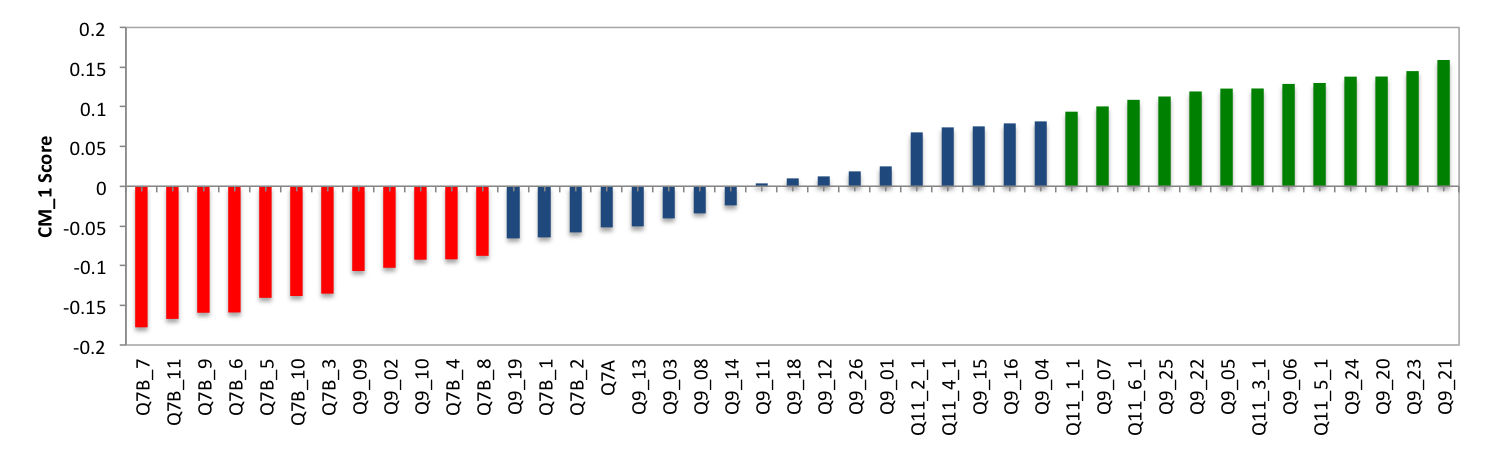
\includegraphics[ width=\textwidth ]{CM1_Cluster0.png}
	\caption{\textbf{CM1 Scores for the 43 questions for Cluster0, based on the
	clustering dataset.} The selected top and bottom questions are shown in red
	and green respectevly.}
	\label{fig:Cluster0}
\end{figure}

The figure ~\ref{fig:Cluster0} demonstrate the CM1 score for the 43
questions for the Cluster0, with the selected 12 lowest and 13 highest ranked
questions shown in red and green respectively. The difference between the
cumulative CM1 socores for Cluster 0 is shown in the figure ???


\begin{figure}[h]
	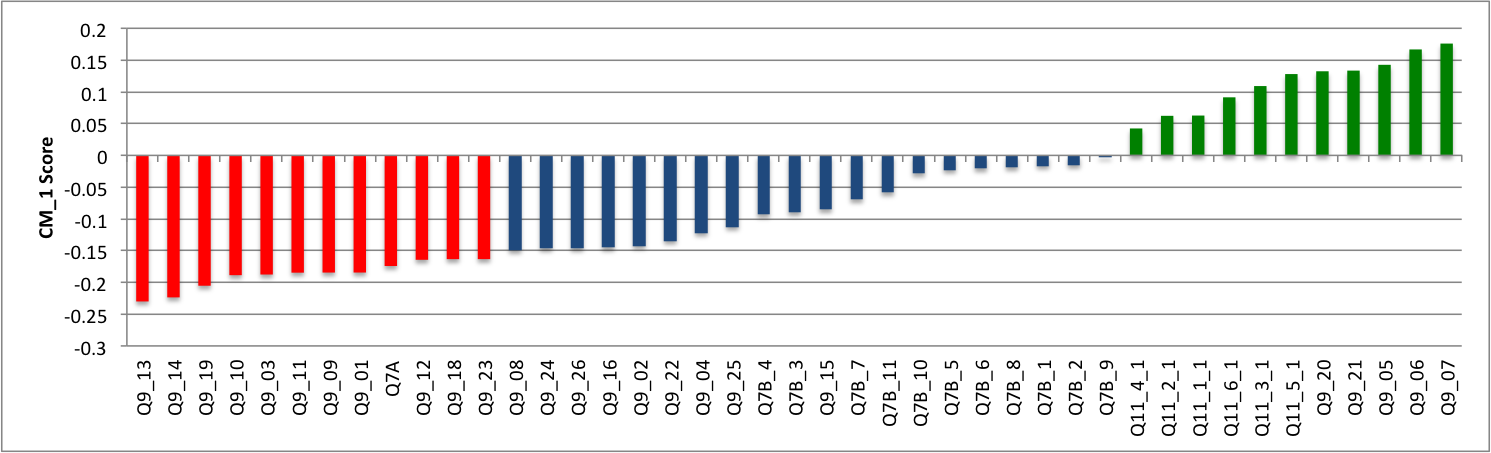
\includegraphics[ width=\textwidth ]{CM1_Cluster1.png}
	\caption{\textbf{CM1 Scores for the 43 questions for Cluster1, based on the
	clustering dataset.} The selected top and bottom questions are shown in red
	and green respectevly.}
	\label{fig:Cluster1}
\end{figure}

\begin{figure}[h]
	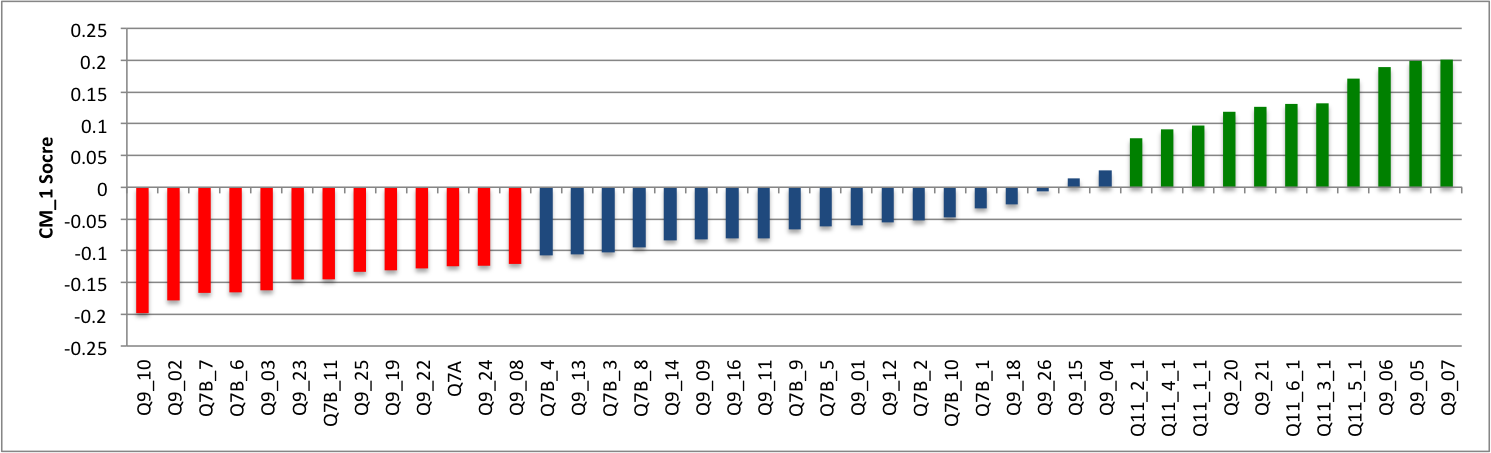
\includegraphics[ width=\textwidth ]{CM1_Cluster2.png}
	\caption{\textbf{CM1 Scores for the 43 questions for Cluster2, based on the
	clustering dataset.} The selected top and bottom questions are shown in red
	and green respectevly.}
	\label{fig:Cluster2}
\end{figure}

\begin{figure}[h]
	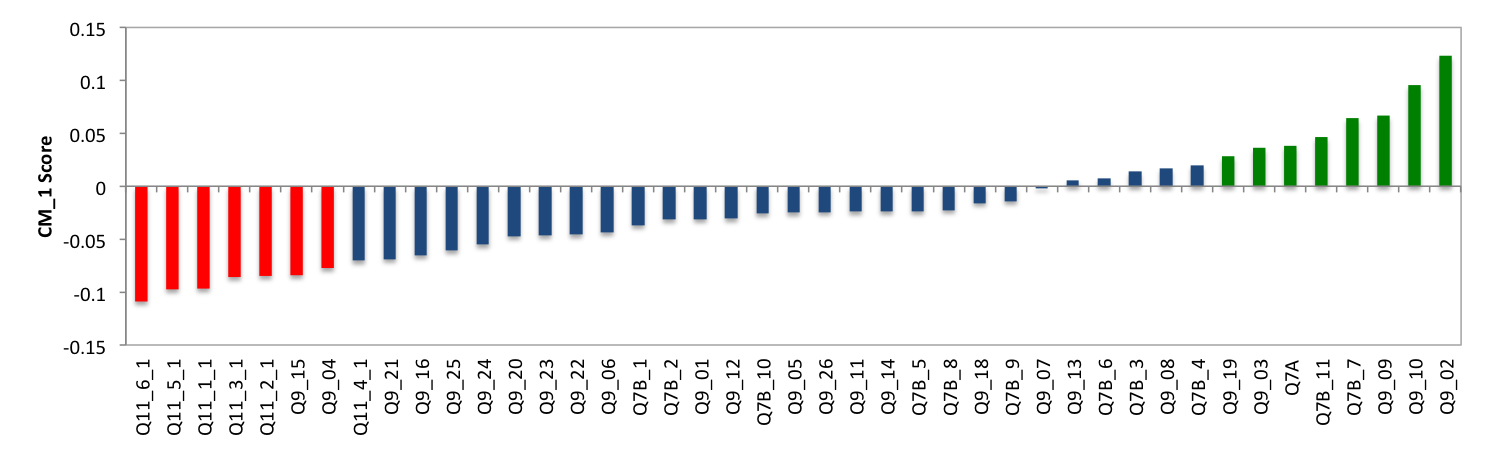
\includegraphics[ width=\textwidth ]{CM1_Cluster3.png}
	\caption{\textbf{CM1 Scores for the 43 questions for Cluster3, based on the
	clustering dataset.} The selected top and bottom questions are shown in red
	and green respectevly.}
	\label{fig:Cluster3}
\end{figure}

\begin{figure}[h]
	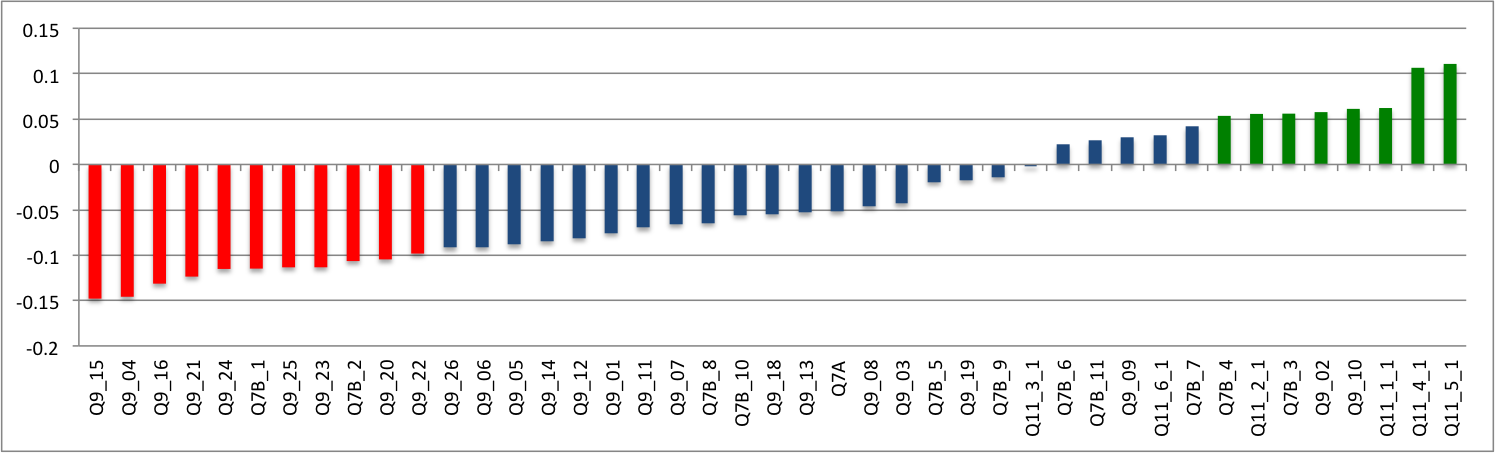
\includegraphics[ width=\textwidth ]{CM1_Cluster4.png}
	\caption{\textbf{CM1 Scores for the 43 questions for Cluster4, based on the
	clustering dataset.} The selected top and bottom questions are shown in red
	and green respectevly.}
	\label{fig:Cluster4}
\end{figure}

\begin{figure}[h]
	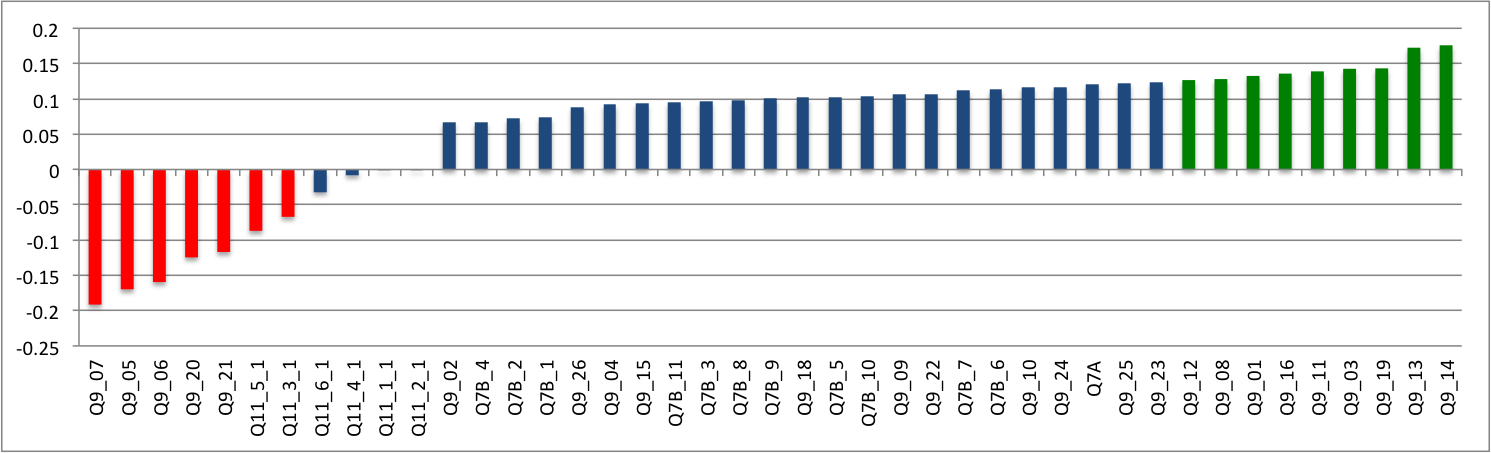
\includegraphics[ width=\textwidth ]{CM1_Cluster5.png}
	\caption{\textbf{CM1 Scores for the 43 questions for Cluster5, based on the
	clustering dataset.} The selected top and bottom questions are shown in red
	and green respectevly.}
	\label{fig:Cluster5}
\end{figure}

\begin{figure}[h]
	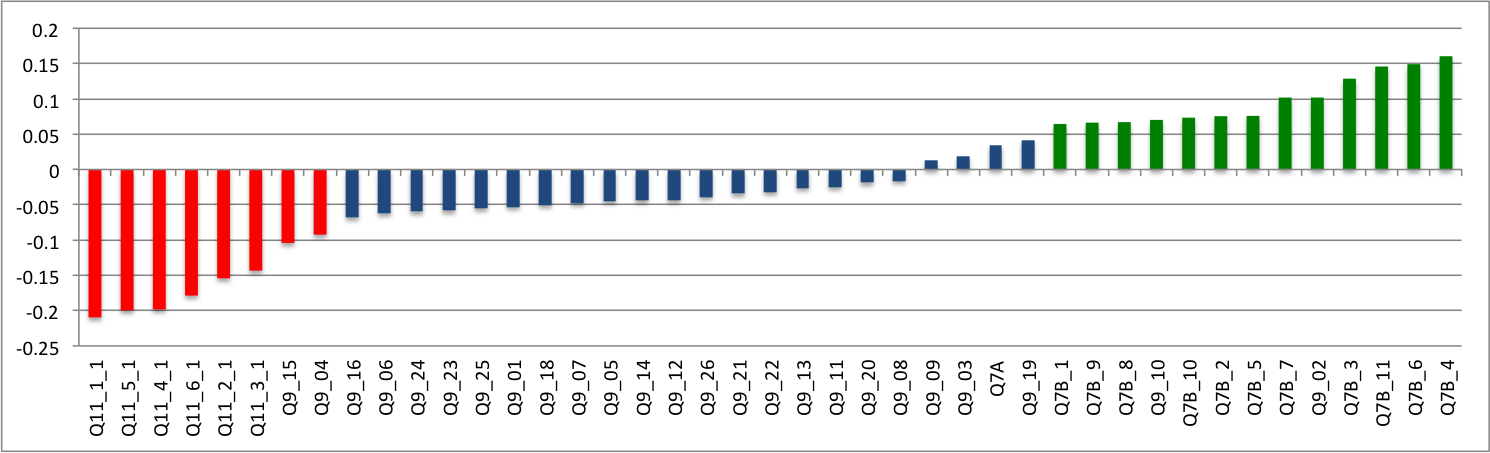
\includegraphics[ width=\textwidth ]{CM1_Cluster6.png}
	\caption{\textbf{CM1 Scores for the 43 questions for Cluster6, based on the
	clustering dataset.} The selected top and bottom questions are shown in red
	and green respectevly.}
	\label{fig:Cluster6}
\end{figure}



\subsubsection{Description of Clusters}

In order to further describe the clusters found by our method, we compute a new
score proposed by(), the CM1 score.



%few sentences on what CM_1 score is
%what does the CM_1 score tell us? (highest vs lowest identifiers of the
% clusters) - get Heloisa's help


\subsection{Discussion and Conclusion}
%(together)

\end{document}

T� funfando? esta ou nao??

